% !TeX root = ../AdaptiveSeedingSTOC.tex

In this section we evaluate the ability of the optimizer to optimize a single parameter in the DFC algorithm with respect to very simple utility functions and budgets. We test the optimizer on both synthetic and real-world datsets and conclude that most of the time it performs as well as the best manual parameter settings. 

\subsection{Methodology}

We evaluate BESTBUY on both Gaussian Random matrices and the Movielens10M dataset (available [HERE]). For each of the two datasets, we divided the available data into several partitions. For the random matrices we used five partitions, and this simply meant one matrix per partition. For the Movielens data (which is one enormous matrix), we partitioned the rows of the matrix into seven pieces. This gave the two datasets a comparable number of nonzero entries per partition. After partitioning the data, we group the partitions into training data and testing data. We used all but one partition for both datasets as training data on which to run DFC computations. The optimizer was then fed the input and output profiles of these computations to use in its database. We used the final partition to test the predictions of the optimizer. Our goal was for the optimizer to automatically choose the degree of parallelism in the DFC algorithm, i.e. how much to slice the input matrix in the Divide step. We asked for the computations to be completed within a specified amount of time while minimizing the error, and DFC computations with manually-chosen parameters designed to meet these budgets were performed on this testing data, as well as a DFC computation with optimizer-chosen division. The evaluation metric we chose was, for each time budget, the error of the optimized parameters compared to the error of the \emph{best} run with manually-chosen parameters. We will see soon that the optimizer performs as well as the best parameter for every budget, even when that parameter changes depending on the budget. Finally, we performed cross-validation, i.e. training and testing was done with each of the partitions used as testing data, and we obtain very consistent results. 

The tests were all performed on the Amazon EC2 Cluster using medium instances. [INSERT SOME MORE DESCRIPTIONS HERE]. 

\subsection{Gaussian Random Matrices}
The first dataset we tested the optimizer on was a synthetic dataset containing many low rank randomly generated matrices. The matrices were generated according to the following procedure: 
\begin{enumerate}
\item Fix parameters $r$, $p$, and $\sigma^2$ which are the rank, percent of revealed entries, and the variance of the noise respectively. In our testing, we used $r = 10$, $p = .1$, and $\sigma^2 = .01$. 
\item Generate two $n \times r$ matrices ${\bf A}$ and ${\bf B}$ with entries drawn from $\mathcal{N}(0,1/\sqrt{r})$. 
\item Let ${\bf N}$ be an $n \times n$ matrix with ${\bf N}(i,j)$ drawn independently from $\mathcal{N}(0,\sigma^2)$. In our dat
\item Define ${\bf M} = {\bf A}{\bf B}^T + {\bf N}$
\item Pick a uniform random subset $\Omega \subset [n] \times [n]$ with $|\Omega| = pn^2$, and let ${\bf M}_{\Omega}$ be the matrix such that ${\bf M}_{\Omega}(i,j) = {\bf M}$ for $(i,j) \in \Omega$ and unknown otherwise. 
\end{enumerate}
This procedure generates a noisy copy of a rank $r$ random matrix whose entries have unit variance and hides most of its entries. Now we can generate many of these matrices and by running a lot of DFC computations for training purposes, we can predict the behavior of DFC on these kinds of instances and thus automatically choose how much to divide the input. 

\begin{figure}
	\begin{subfigure}[b]{.45\textwidth}
\begin{center}
		\fbox{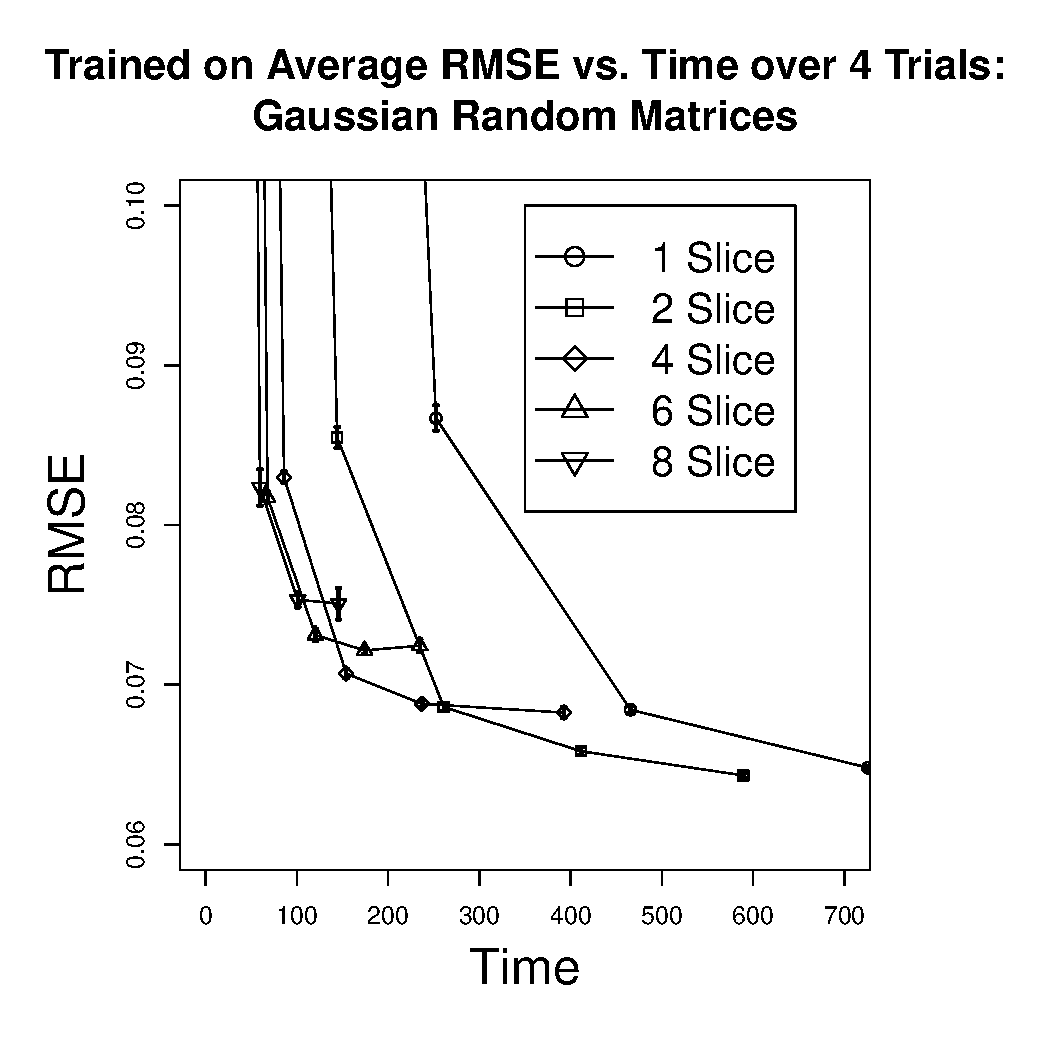
\includegraphics[width=\textwidth]{Graphs/4000_90_1_to_4_RvT_graph.pdf}}
		\caption{Training Data.}
\end{center}
	\end{subfigure}
\hspace{1cm}
	\begin{subfigure}[b]{.45\textwidth}
\begin{center}
		\fbox{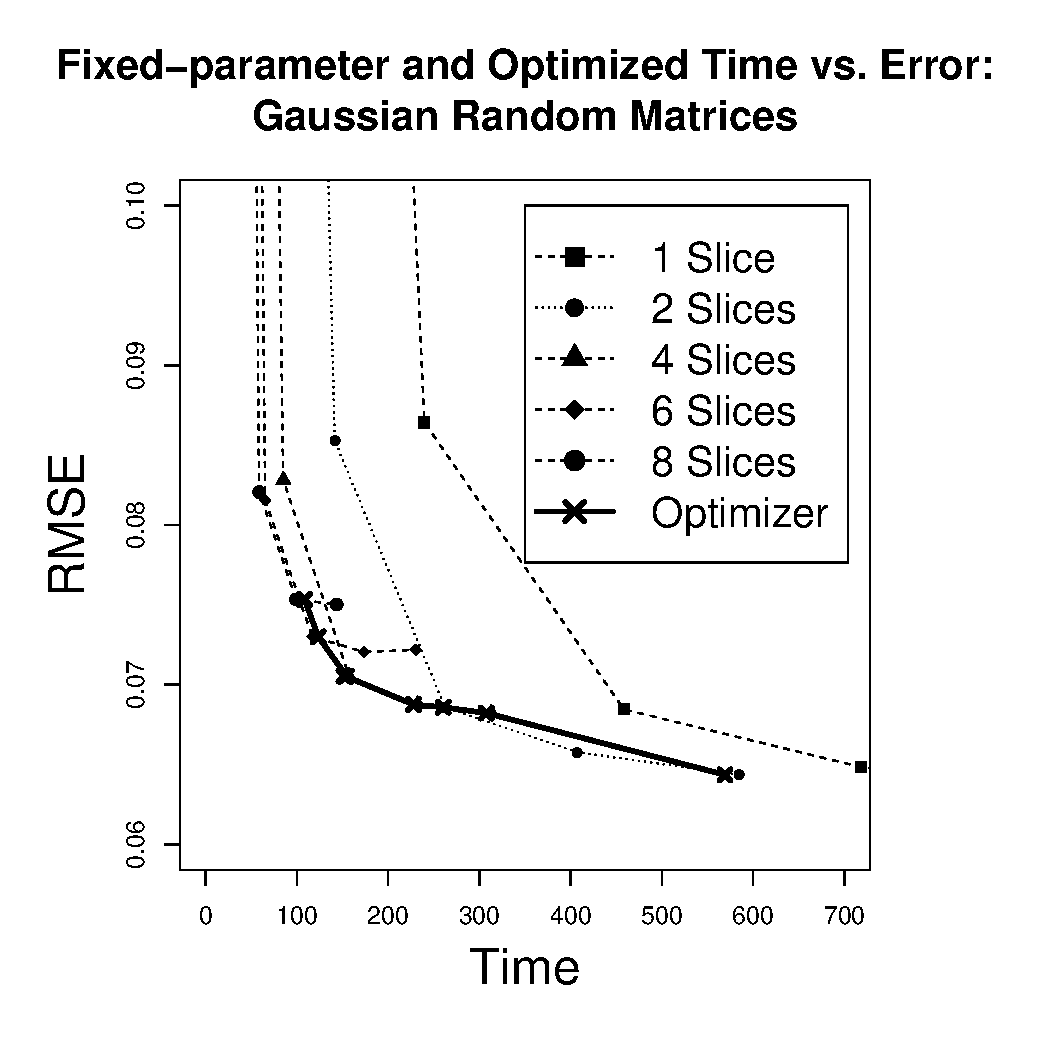
\includegraphics[width=\textwidth]{Graphs/Opt_Gaussian_4000.pdf}}
		\caption{Testing Data.}
\end{center}
	\end{subfigure}
\hfill
	\caption{Plots of Time and Error taken to factor a 4000 by 4000 matrix drawn from a Gaussian distribution.}	
\end{figure}